\subsection*{Teil D: Rationale Zahlen und Textaufgaben (25 Minuten)}

\begin{enumerate}[resume, label=\arabic*.]
    \item \textbf{Rechne mit negativen Zahlen:}

    \begin{enumerate}[label=\alph*)]
        \item $(-3) + 5 = $ \underline{\hspace{3cm}}
        \item $2 - 7 = $ \underline{\hspace{3cm}}
        \item $(-4) + (-2) = $ \underline{\hspace{3cm}}
        \item $(-5) - (-3) = -5 + 3 = $ \underline{\hspace{3cm}}
    \end{enumerate}

    \vspace{0.5cm}

    \item \textbf{Kontostand:}

    Max hat 25 € auf seinem Konto. Er hebt 30 € ab.

    \begin{enumerate}[label=\alph*)]
        \item Wie ist sein neuer Kontostand? 
        $25 - 30 = $ \underline{\hspace{3cm}} €

        \item Er zahlt dann 15 € ein. Kontostand jetzt? 
        \underline{\hspace{2cm}} € $+ 15$ € = \underline{\hspace{3cm}} €
    \end{enumerate}

    \vspace{0.5cm}

    \item \textbf{Mischungsaufgabe:}

    Für einen Obstsalat mischt Lisa:
    \begin{itemize}
        \item $\dfrac{1}{2}$ kg Äpfel
        \item $\dfrac{1}{4}$ kg Birnen  
        \item $\dfrac{3}{4}$ kg Trauben
    \end{itemize}

    \begin{enumerate}[label=\alph*)]
        \item Wie viel kg Obst hat sie insgesamt?

        $\dfrac{1}{2} + \dfrac{1}{4} + \dfrac{3}{4} = \dfrac{2}{4} + \dfrac{1}{4} + \dfrac{3}{4}$ = \underline{\hspace{3cm}} kg

        \item Welchen Anteil machen die Äpfel aus?

        $\dfrac{\text{Äpfel}}{\text{Gesamt}} = \dfrac{1/2}{\phantom{3/2}}$ = \underline{\hspace{3cm}}
    \end{enumerate}

    \vspace{0.5cm}

    \item \textbf{Prozent und Diagramm:}

    In einer Umfrage zur Schulweg:
    \begin{itemize}
        \item 30\% kommen mit dem Bus
        \item 45\% kommen zu Fuß
        \item Rest kommt mit dem Fahrrad
    \end{itemize}

    \begin{enumerate}[label=\alph*)]
        \item Wie viel Prozent kommen mit dem Fahrrad? 
        $100\% - 30\% - 45\% = $ \underline{\hspace{3cm}}

        \item Bei 40 Schülern: Wie viele kommen zu Fuß? 
        $45\%$ von 40 = $\dfrac{45}{100} \cdot 40$ = \underline{\hspace{3cm}} Schüler

        \item Zeichne ein einfaches Säulendiagramm:

        \begin{center}
            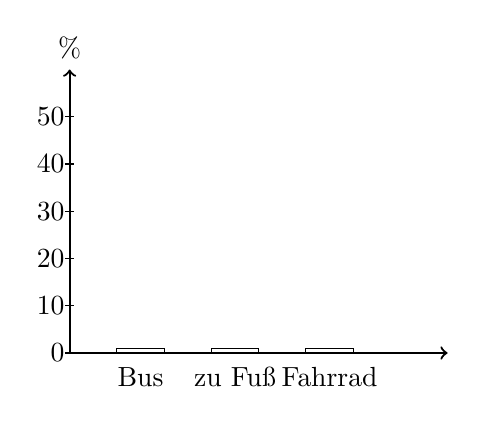
\begin{tikzpicture}[scale=0.6]
                \draw[thick,->] (0,0) -- (0,6) node[above] {\%};
                \draw[thick,->] (0,0) -- (8,0);
                \foreach \y in {0,10,20,30,40,50}
                \draw (-0.1,\y/10) -- (0.1,\y/10) node[left] {\y};
                \node at (1.5,-0.5) {Bus};
                \node at (3.5,-0.5) {zu Fuß};
                \node at (5.5,-0.5) {Fahrrad};
                \draw (1,0) rectangle (2,0.1);
                \draw (3,0) rectangle (4,0.1);
                \draw (5,0) rectangle (6,0.1);
            \end{tikzpicture}
        \end{center}
    \end{enumerate}

    \vspace{0.5cm}

    \item \textbf{Abschlussaufgabe - Pizzaparty:}

    Für eine Party werden 8 Pizzen bestellt. Jede Pizza wird in 8 Stücke geschnitten.

    \begin{enumerate}[label=\alph*)]
        \item Wie viele Stücke gibt es insgesamt? 
        $8 \cdot 8 = $ \underline{\hspace{3cm}} Stücke

        \item 20 Kinder essen je 2 Stücke, 4 Erwachsene je 3 Stücke.
        Wie viele Stücke werden gegessen?
        $(20 \cdot 2) + (4 \cdot 3) = 40 + 12 = $ \underline{\hspace{3cm}} Stücke

        \item Welcher Bruchteil der Pizzen bleibt übrig?
        \begin{itemize}
            \item Übrige Stücke: $64 - 52 = $ \underline{\hspace{2cm}} Stücke
            \item Als Bruchteil: $\dfrac{12}{64} = \dfrac{3}{16}$ der Pizzen
        \end{itemize}

        \item Jede Pizza kostet 7,50 €. Was kosten alle Pizzen?
        $8 \cdot 7,50$ € = \underline{\hspace{3cm}} €
    \end{enumerate}
\end{enumerate}